An actor network that represents the video filter application is constructed in PREESM. The final PiSDF model of the PREESM video filter application is presented in figure \ref{fig:preesm_actors}. The PREESM filter application is adapted from the PREESM example in \cite{preesmtut} by adding another processing path for the gaussian filter and making the necessary modifications to the shared parts of the application.

\begin{figure}[h!]
    \begin{center}
        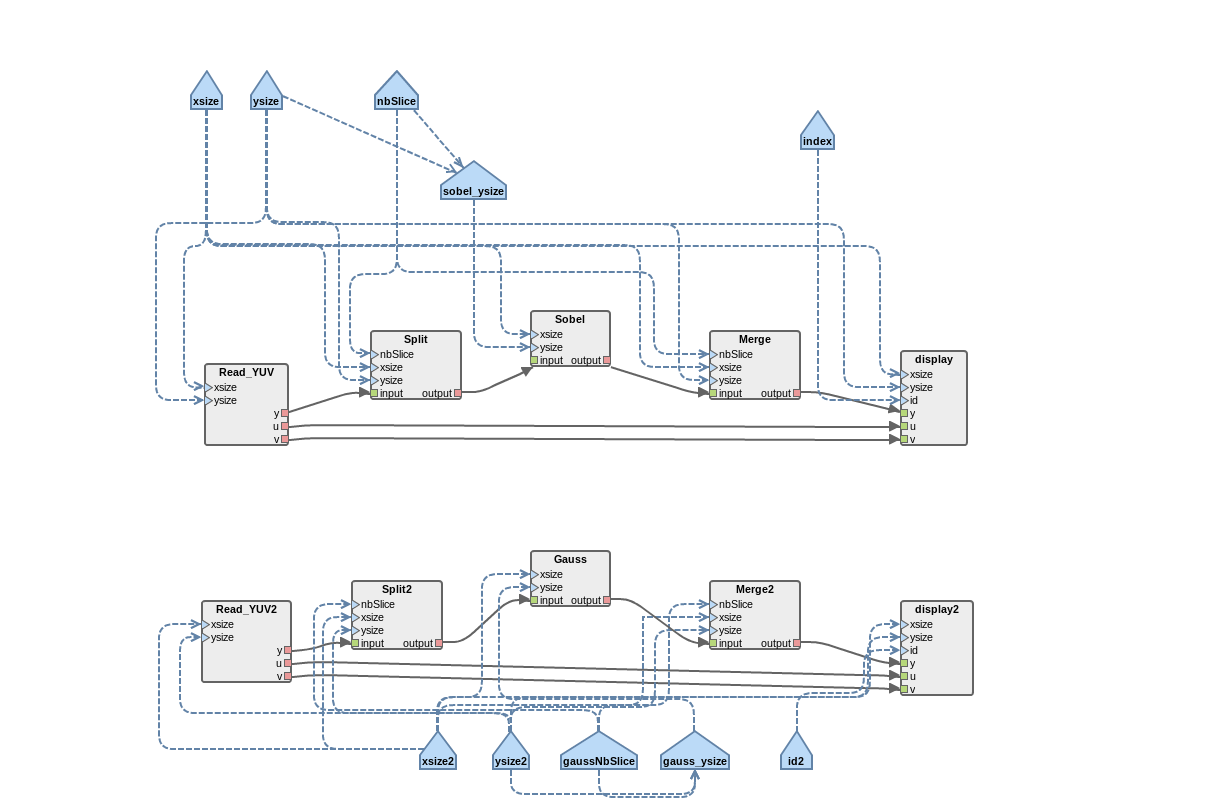
\includegraphics[width=0.99\textwidth]{images/preesm_diagram.png}
        \caption{The PiSDF graph of the PREESM filter application}
        \label{fig:preesm_actors}
    \end{center}
\end{figure}

\subsection{The Actor Model}
\label{subsec:actors}
To keep the model simple and the program well analyzable both of the processing paths in the network are independent. The first actor on both of the processing paths, the Read\_YUV and the Read\_YUV2 actors in the figure \ref{fig:preesm_actors}, loads the video frames from memory and passes them to splitting actors. The splitting actors split the frames to a suitable number of splices to enable processing of the same video stream on multiple cores. The filter actors, Sobel and Gauss actors in the figure, follow the splitting actors. Partial frames filtered in the filter actor are merged back to whole frames in the merge actors. The last actors on both of the processing paths are dummy actors. The pentagons in the top and the bottom of the figure represent the parameters of the application. The \texttt{xsize}, \texttt{ysize}, \texttt{xsize2} and \texttt{ysize2} parameters specify the size of the input frames. \texttt{nbSlice} and \texttt{gaussNbSlice} determine the numbers of slices the frames are split to. The \texttt{sobel\_ysize} and \texttt{gauss\_ysize} are the heights of the slices after splitting.

The first actors Read\_YUV and Read\_YUV2 call the \texttt{readYUV} function defined in the PREESM example at \cite{preesmtut}. As I/O is not in the scope of the experiments it is omitted from the application. The processing starts with loading the frames from memory. In a real world application the frames would be written to the memory for example with DMA by a packet processor processing a stream of network packets. The \texttt{readYUV} function copies the Y component of the input frame to the output address while the U and V components are ignored. The U and V are omitted because the sobel and gauss actors only operate on the Y channel in the experiment setup.

The split actor operates on the output of the Read\_YUV actor. The split actor preprocesses the frame for the sobel and gauss actors. Since the sobel and gauss filters involve convolution with 3x3 and 5x5 matrices respectively, they will need to access image data outside the part of the image they are processing. To enable parallel processing of a single frame on multiple cores, the frame is split in to slices. These slices will also need to contain a bit of extra data so that the filters can operate correctly. Black lines, or lines with the Y value of 0 are added to the top and the bottom of the frame. One black line is enough for the sobel frames but two black lines are needed for the gaussian frames, corresponding to the filter kernel sizes. After the padding, the slices overlap each other for one or two lines again corresponding to the size of the filter kernel. With the black lines added the frame is copied to the output buffer one slice at a time. 

The sobel actor calculates the convolution of the sobel kernels in presented in \ref{fig:sobelmat} with the Y component of the input frame. The sobel actor from from the PREESM example at \cite{preesmtut} is used in this experiment as well. The convolution is computed by looping over the pixels in the input frame, calculating the $G_{x}$ and $G_{y}$ components of the sobel operator and combining them by computing the average of absolute values of $G_{x}$ and $G_{y}$. After looping over the image the actor overwrites the edges of the frame with black pixels.

The gauss actor operates similarly to the sobel actor but instead of closed expressions the value of the filter function at each points is calculated by looping over the neighboring pixels and multiplying the intensity values by the corresponding weight from the gaussian kernel presented in \ref{fig:gaussmat}.

The last actor processing the frame is the merge actor. The merge actor copies the processed data from its input buffer to its output buffer, overlaying the slices so that the output frame doesn't contain the extra lines created in the split actor. Since there is no real I/O in the application, the merged frame is not processed further. In a real world application the processed frame would be copied for example to a network packet. As there is no I/O the display actors don't do any computations. In the experiments the display actor is used as the endpoint of the processing and it starts the data export.

\subsection{The PREESM Schedule}
\label{subsec:preesmsched}
The scheduler in the PREESM framework is described in \ref{sec:preesm-scheduling}. The scheduler creates a block schedule from the actor model using user provided estimates for the actor durations. To get reasonably accurate estimates, the application was first scheduled with the default values and the actor durations were measured on the target device. The resulting timings are presented in the table \ref{tab:preesm_times}. The timings from the measurements were approximately the same for all the actors except for the gauss actor. A gantt chart representing the schedule created using the values in the table is presented in figure \ref{fig:preesm_gantt}. The mutable parameters in the graph \ref{fig:preesm_actors} affect the static memory allocations of the PREESM application and the PREESM codegen workflow needs to be executed every time the parameters are changed. Because of this the PREESM schedules of the different measurement setups are slightly different.

\begin{table}
    \begin{center}
        \begin{tabular}{| c | c |}

            \hline
            Cycles & Actor \\ \hline
            600 & Gauss \\ \hline
            150 & Merge \\ \hline
            150 & Merge2 \\ \hline
            150 & Read\_YUV \\ \hline
            150 & Read\_YUV2 \\ \hline
            150 & Sobel \\ \hline
            150 & Split \\ \hline
            150 & Split2 \\ \hline
            1 & display \\ \hline
            1 & display2 \\ \hline
        \end{tabular}
        \caption{PREESM Actor Timings.}
        \label{tab:preesm_times}
    \end{center}
\end{table}

The PREESM framework doesn't support changing the timing of the implode and explode operations which started affecting the schedule considerably with larger frame sizes. The duration estimates used by PREESM for the implode and explode operations are very short compared to durations of the actors measured from the application. The explode operations for both streams are represented in the gantt chart by the small time slices predecing gauss actors on cores 4 and 7. The implode operation for gauss stream follows the gauss actor execution on core 7 and the implode operation of sobel stream follows the latter sobel actor on core 5.

\begin{figure}[h!]
    \begin{center}
        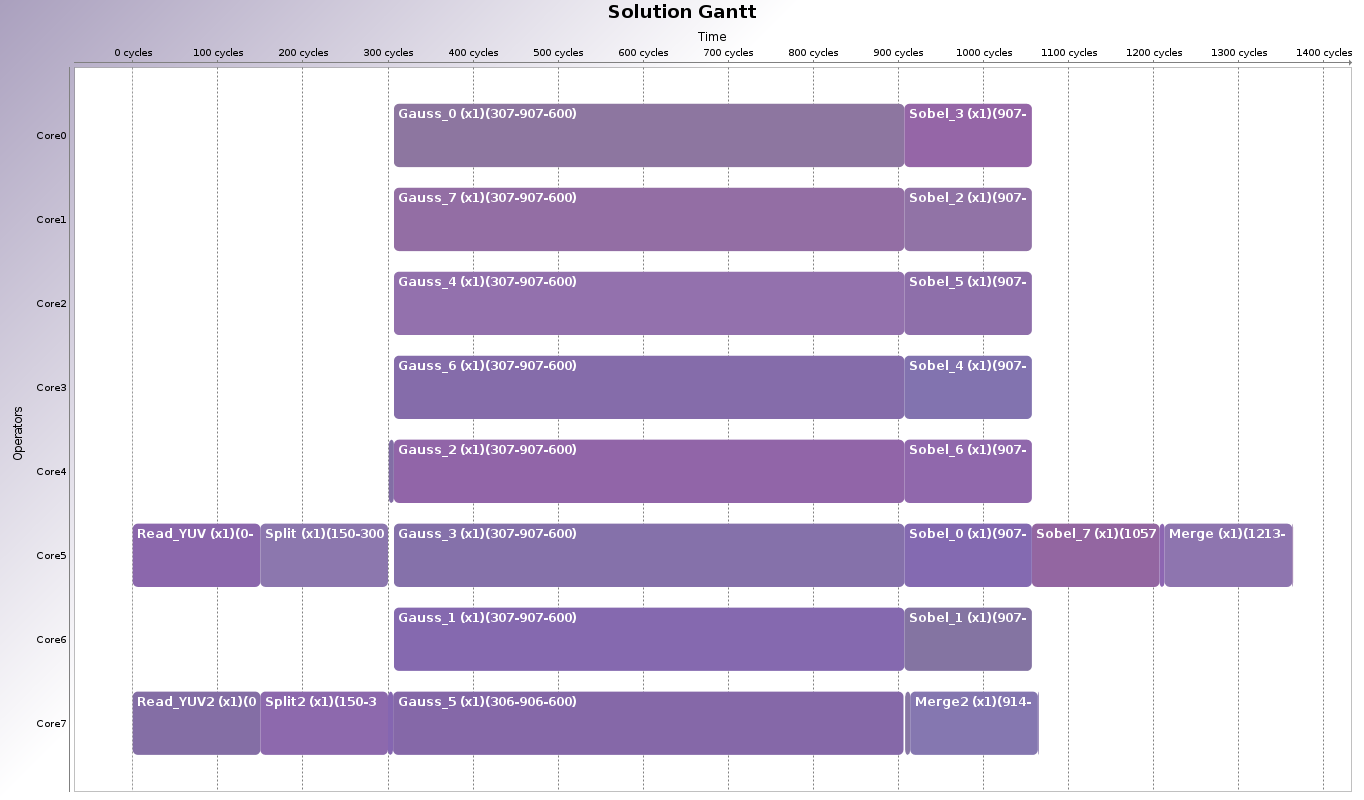
\includegraphics[width=0.99\textwidth]{images/gantt_preesm_cifcif.png}
        \caption{Gantt chart representing the schedule of a PREESM Filter Application.}
        \label{fig:preesm_gantt}
    \end{center}
\end{figure}

A block schedule could be generated, which would yield a higher throughput by introducing multiple instances of the actors for each repetition of the schedule. The successive repetitions of the schedule would be interleaved and the overhead of synchronizing the cores would be reduced. The current version of PREESM does not support the described interleaving of the repetitions \cite{pelcat2014preesm}.
